\subsection{Is Aging Necessary?}

% \begin{frame}[c]{Animals that do not senescence (age)}
%     \large
%     \begin{itemize}[<+(1)->]
%         \item hydra (biologically immortal) \cite{martinez1998mortality}
%         \item naked mole rats \cite{ruby2018naked}
%         \item tortoises \cite{miller2001escaping}
%         \item some sharks: 400y \cite{Greenlan67:online}
%         \item some clams: 500y \cite{munro2012extreme}
%         % \item whales
%     \end{itemize}
%     \pause
%     Conclusion: Biological creatures don't {\em have} to age
% \end{frame}

\begin{frame}[c]{Animals that do not Age}
    \scriptsize
    \begin{multicols}{2}
        % trim = l b r t
        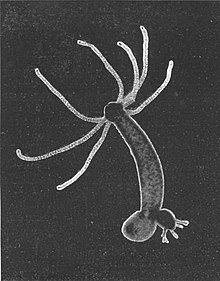
\includegraphics[width=0.35\textwidth,clip,trim=0 30 0 40]{hydra} \\
        Hydra (biologically immortal) \cite{martinez1998mortality} \\
        \pnote{
            Hydras don't age and could live forever \\
            if not eaten or otherwise killed before that \\
            Keyword: Mortality does not increase with age \\
        }
        \pause

        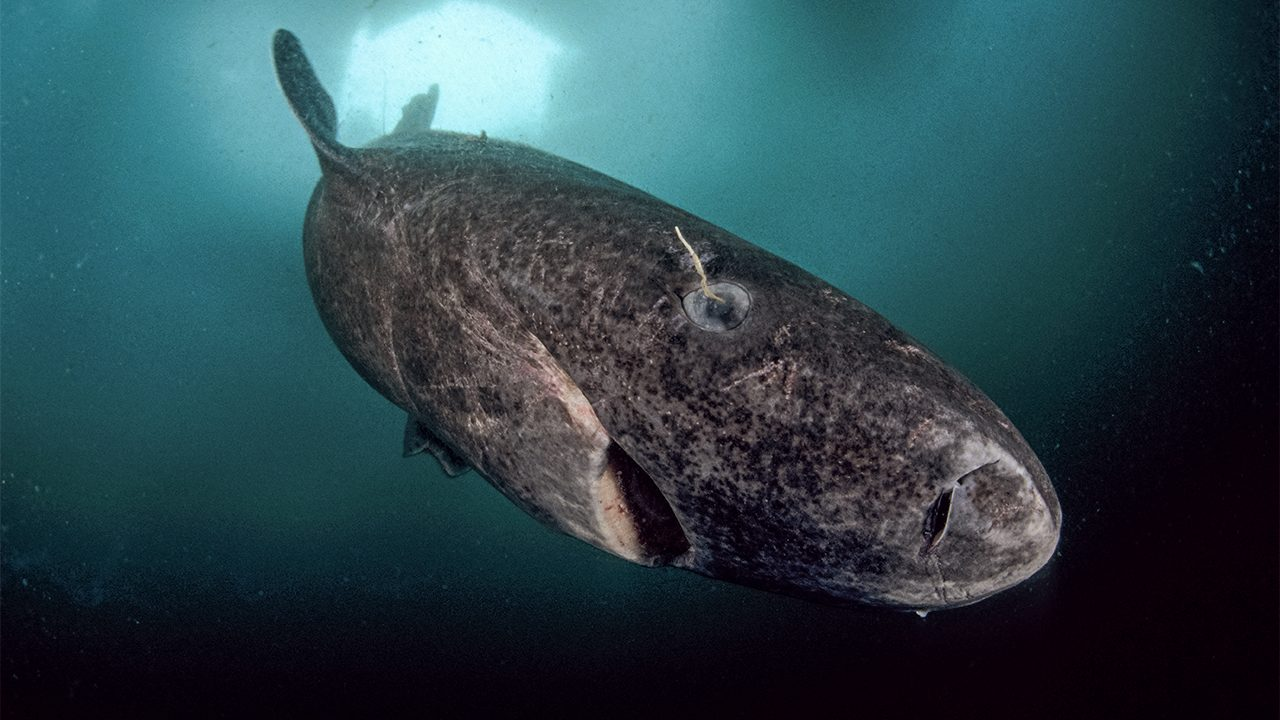
\includegraphics[width=0.35\textwidth,clip,trim=0 90 0 30]{shark} \\
        Greenland sharks: 400y \cite{Greenlan67:online} \\
        \pnote{
            These sharks also don't age biologically \\
            biologically indistinguishable regarding age \\
            still eventually die, but we don't know why \\
        }
        \pause

        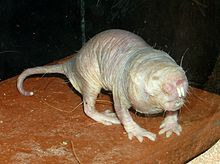
\includegraphics[width=0.35\textwidth,clip,trim=0 25 0 25]{nacktmull} \\
        Naked Mole Rats \cite{ruby2018naked},
        Picture (CC BY-SA 3.0): \cite{Nacktmul31:online} \\
        \pnote{
            Similar story with these Naked Mole Rats \\
            researched better, pot. mechanisms found \\
            maybe ask me in the Q&A \\
        }
        \pause

        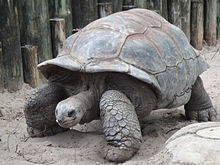
\includegraphics[width=0.35\textwidth]{turtoise} \\
        Tortoises \cite{miller2001escaping},
        Picture (CC BY-SA 3.0): \cite{Tortoise98:online} \\
        \pnote{
            Some Tortoises same, don't age biologically
        }
    \end{multicols}
    \pause
    % \large
    \normalsize
    Conclusion: Biological creatures don't {\em have} to age
\end{frame}



\begin{frame}[c]{Extending Life in different Animals}
    \scriptsize
    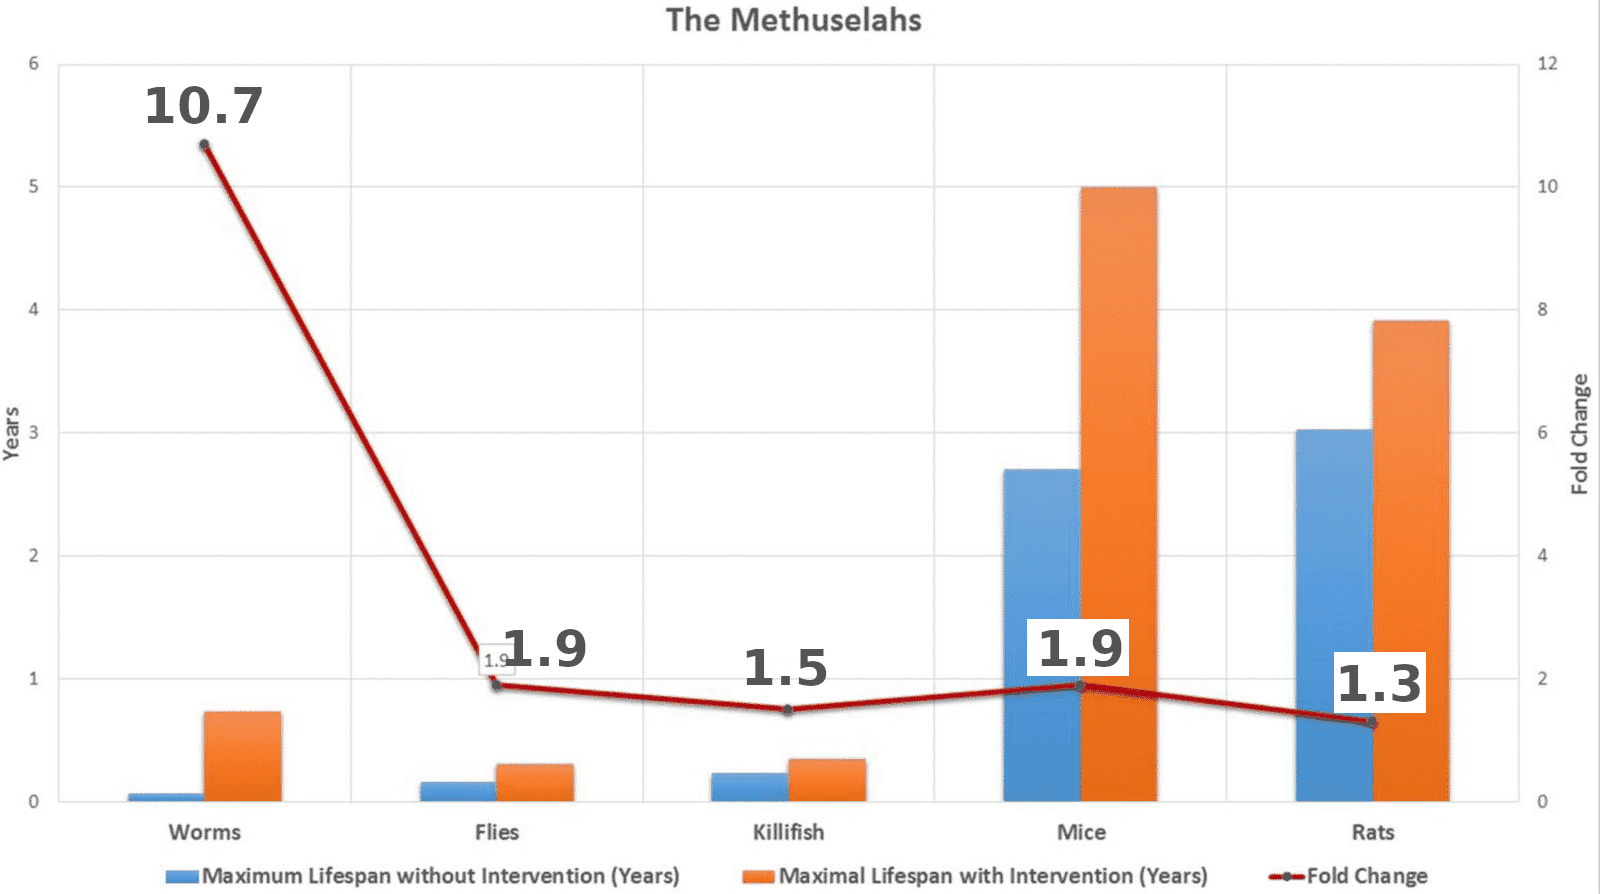
\includegraphics[width=\textwidth]{extending_life} \\
    Source: \cite{bulterijs2015time}
    \pnote{
        We have been successful in extending life \\
        in different species. Rats: 1.89 recently \\
        \par
        We have shown it in animals, no reason \\
        to assume it wouldn't work in humans \\
    }
    \pause
    \large
    It is possible to extend biological Lifespan!
\end{frame}
